\documentclass[xcolor={table}]{beamer}
\usetheme{Singapore}
\usepackage[utf8]{inputenc}
\usecolortheme{crane}
\usepackage{graphicx}
\usepackage{iwona}
\usepackage{standalone}
\usepackage{tikz}
\usetikzlibrary{arrows}
\usetikzlibrary{decorations.markings}
\usetikzlibrary{calc}
\usetikzlibrary{shapes,snakes}
\usepackage{amsmath}
\usepackage{amsfonts}
\usepackage{amsthm}
\usepackage{mathtools}
% \usepackage{minted}
% \usemintedstyle{trac}

\definecolor{lightblue}{RGB}{124,190,255}
\definecolor{darkgreen}{RGB}{24,145,0}

\beamertemplatenavigationsymbolsempty
\setbeamerfont{caption}{size=\tiny}


\title{Deadlock in Queueing Networks}
\author{Geraint Palmer\newline \scriptsize{Paul Harper, Vincent Knight}}
\date{CORS 2016 - Banff}
\titlegraphic{
\includegraphics[width=1.5cm]{../cflogo.pdf}}

\begin{document}
\frame{\titlepage}


% 1st slide, ABUHB, some facs & figures
\begin{frame}
\frametitle{Aneurin Bevan University Health Board}
\begin{figure}

\includegraphics[width=0.45\textwidth]{img/ABUHBlogo}\\
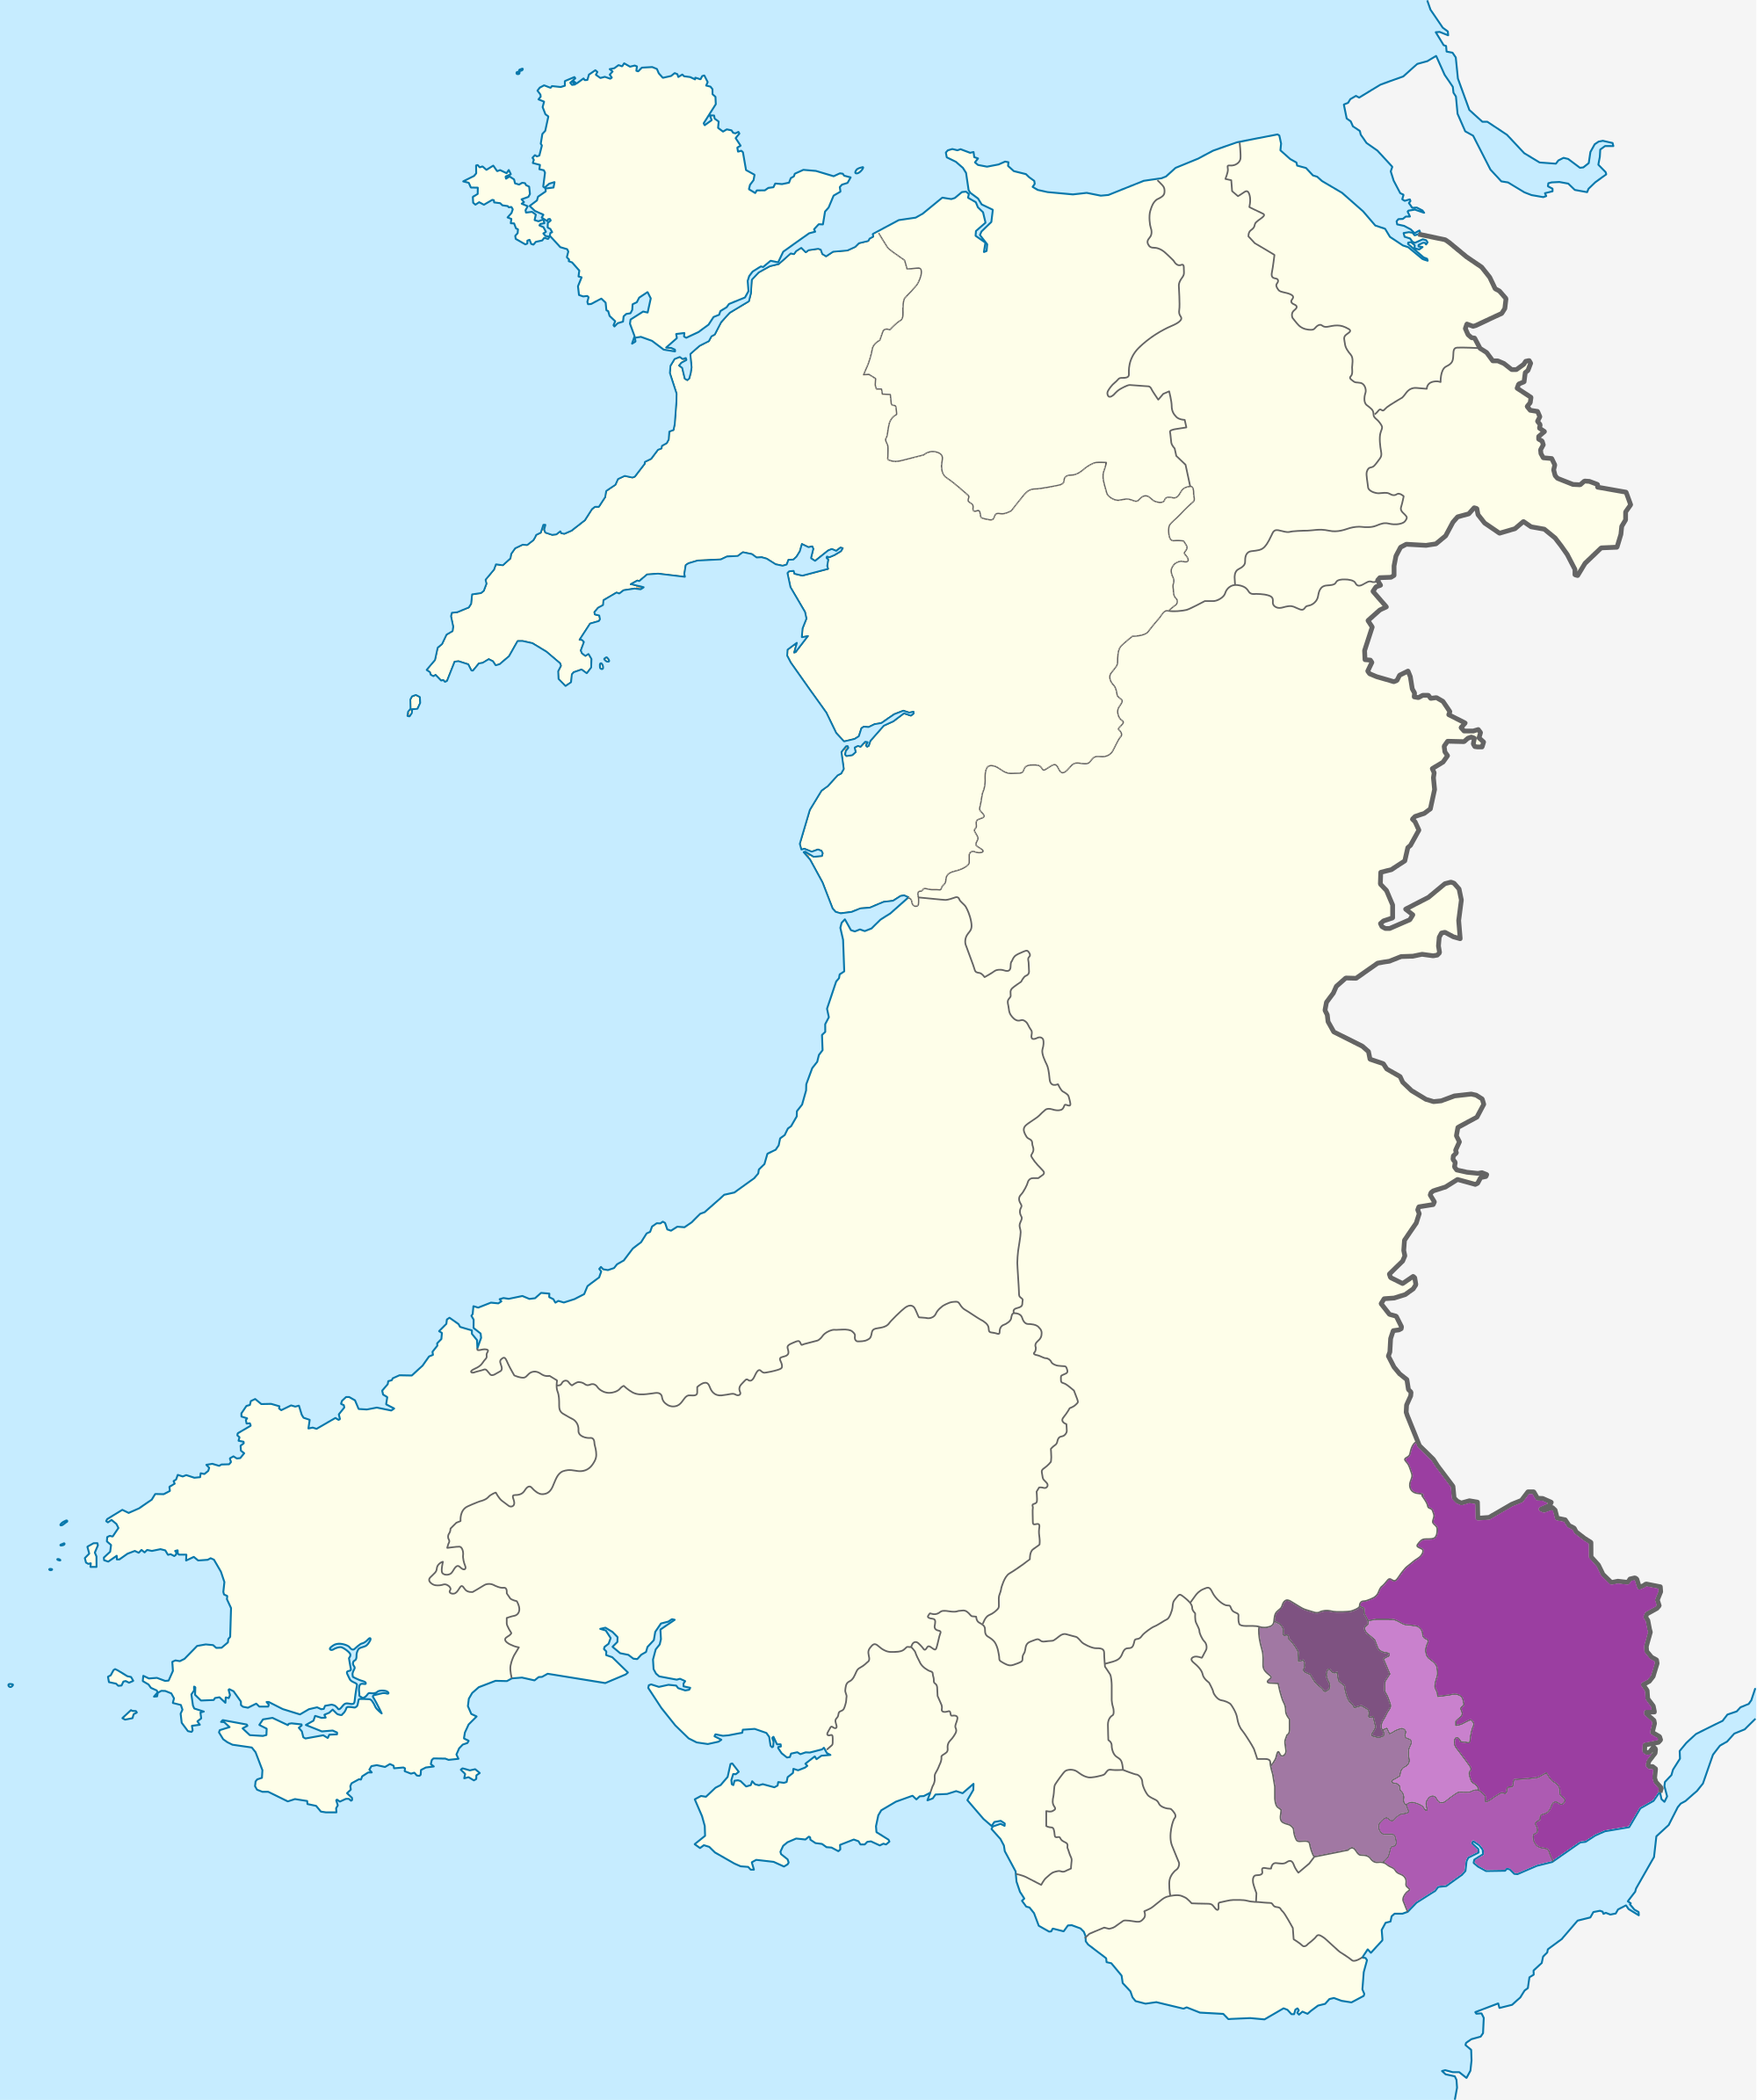
\includegraphics[width=0.45\textwidth]{img/Aneurin_Bevan_all_Wales}
\end{figure}
\end{frame}

\begin{frame}
\frametitle{Elderly People's Flows Through Health System}
\begin{figure}
\includestandalone[width=\textwidth]{img/patient_flows}
\end{figure}
\end{frame}

\begin{frame}
  \frametitle{Deadlock}
    \begin{figure}
    \includestandalone[width=0.7\textwidth]{img/gridlock}
    \end{figure}
\end{frame}

\begin{frame}
\includestandalone[width=\textwidth]{img/2nodefeedbackexample}
\end{frame}

\begin{frame}
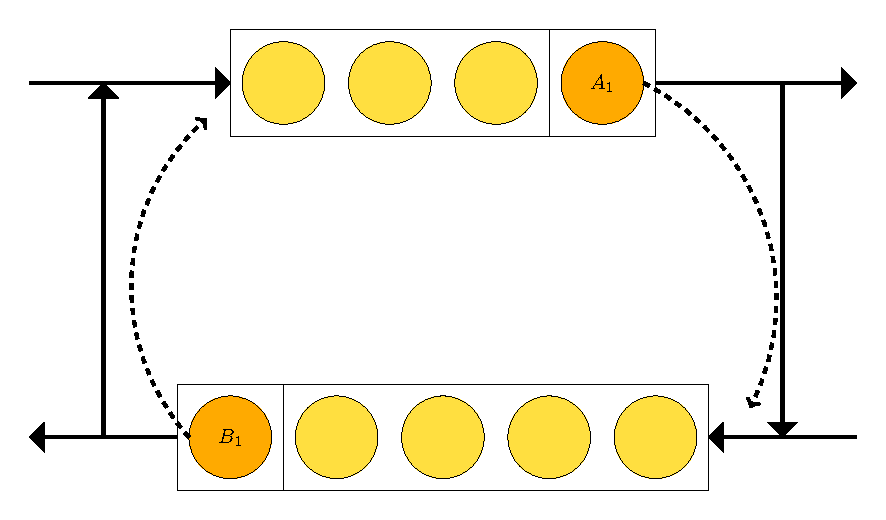
\includegraphics[width=\textwidth]{img/2nodesindeadlock.pdf}
\end{frame}


% 6th slide, digraph and detecting deadlock with knots
\begin{frame}
    \begin{figure}
    \includestandalone[width=\textwidth]{img/buildupdigraph}
    \end{figure}
\end{frame}

% % 7th slide, deadlock detection within Ciw
% \begin{frame}
% \frametitle{Deadlock Detection in Ciw}
% \begin{center}
% \fontsize{8.5pt}{10pt} \inputminted{python}{deadlockciw.py}
% \end{center}
% \end{frame}

% 8th slide, introduce 3 deadlocking networks that will be investigated
\begin{frame}
\frametitle{Three Deadlocking Queueing Networks}
\begin{figure}
\includestandalone[width=\textwidth]{img/3networks}
\end{figure}
\end{frame}

% 9th slide, Markovian deadlock model 1 Node
\begin{frame}
    \frametitle{Markovian Model of Deadlock}
    \includestandalone[width=\textwidth]{img/1nodemultiserver}\newline
    \center{\LARGE{$(i)$}}
\end{frame}

\begin{frame}
\center
\scriptsize  \[S = \{i\in\mathbb{N} \nonscript\; | \nonscript\; 0 \leq i \leq n + 2c\}\]
Define $\delta = i_2 - i_1$\newline

\vspace{10 mm}

  $  q_{i_1, i_2} = \left\{
  \begin{matrix*}[ r ]
    \left. \begin{matrix*}[ r ]
      \color{red} \Lambda & \color{red} \text{if } \delta = 1 \\
      \color{blue} (1-r_{11})\mu\text{min}(i, c) & \color{blue} \text{if } \delta = -1 \\
      0 & \text{otherwise}
    \end{matrix*} \right\} & \text{if } i_1 < n + c \\
  \end{matrix*} \right.
$
\vspace{10 mm}

  $q_{i_1, i_2} = \left\{
  \begin{matrix*}[ r ]
    \left. \begin{matrix*}[ r ]
      \color{darkgreen} (c-b)r_{11}\mu & \color{darkgreen} \text{if } \delta = 1 \\
      \color{blue} (1-r_{11})(c-b)\mu & \color{blue} \text{if } \delta = -b-1\\
      0 & \text{otherwise}
    \end{matrix*} \right\} & \text{if } i_1 = n + c + b \\
  \end{matrix*} \right.
  \quad \forall \quad 0 \leq b \leq c$

\vspace{10 mm}
\end{frame}

\begin{frame}
    \begin{figure}
    \includestandalone[width=0.95\textwidth]{img/MC1nodemultiserv}
    \end{figure}
\end{frame}

\begin{frame}
    \frametitle{Times to Deadlock}
    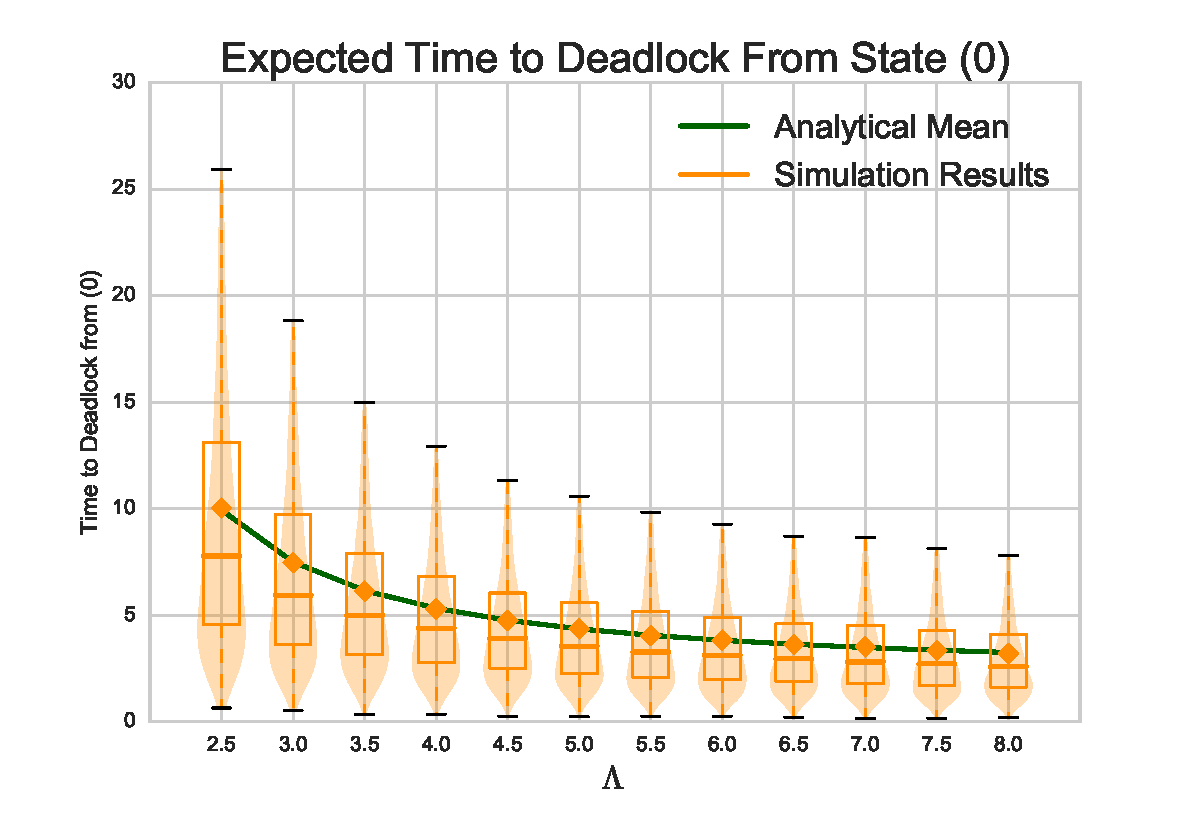
\includegraphics[width=0.5\textwidth]{img/varyL_1Nms}
    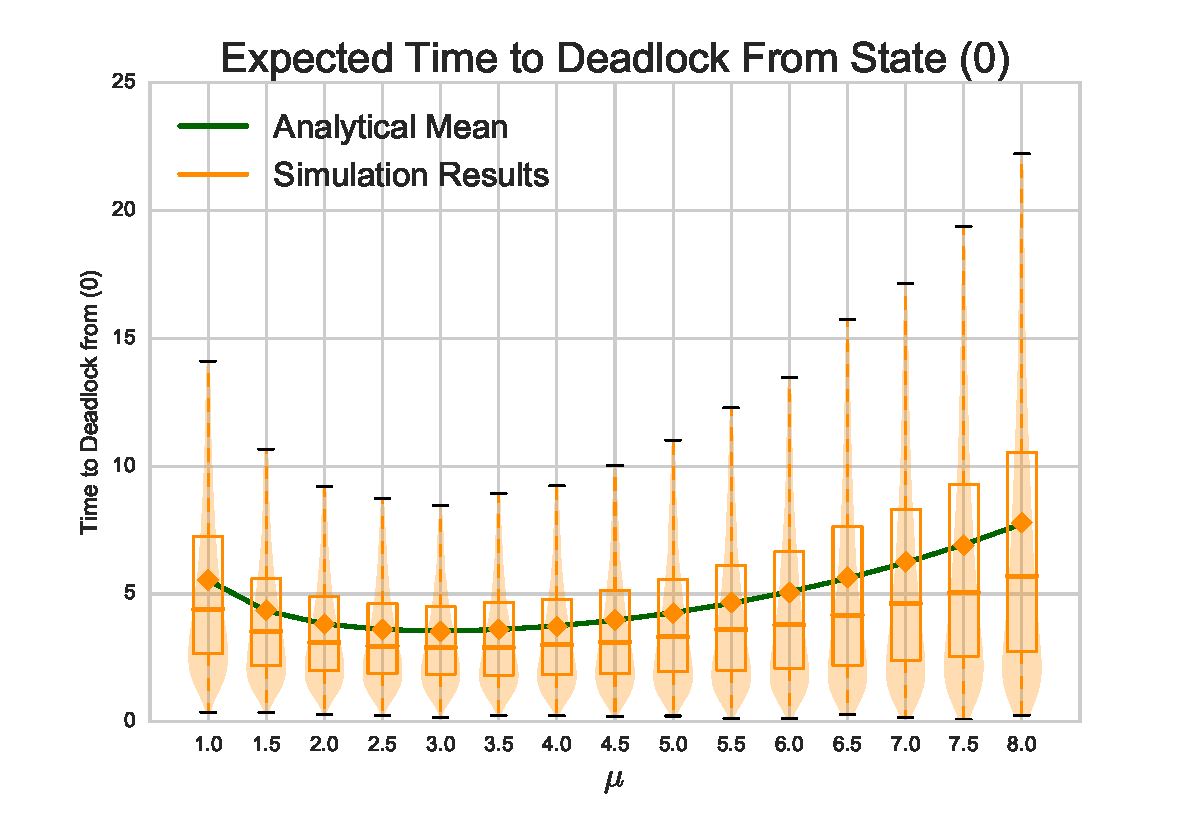
\includegraphics[width=0.5\textwidth]{img/varymu_1Nms}\newline
    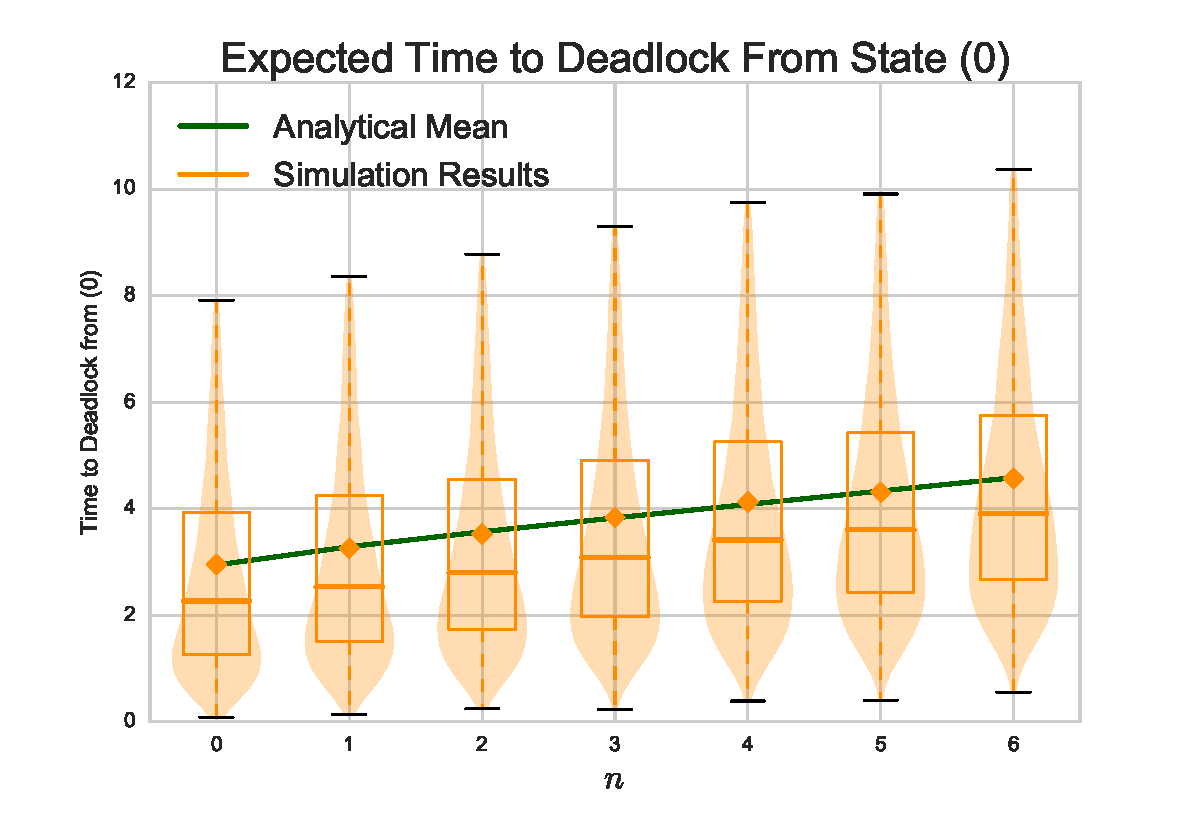
\includegraphics[width=0.5\textwidth]{img/varyn_1Nms}
    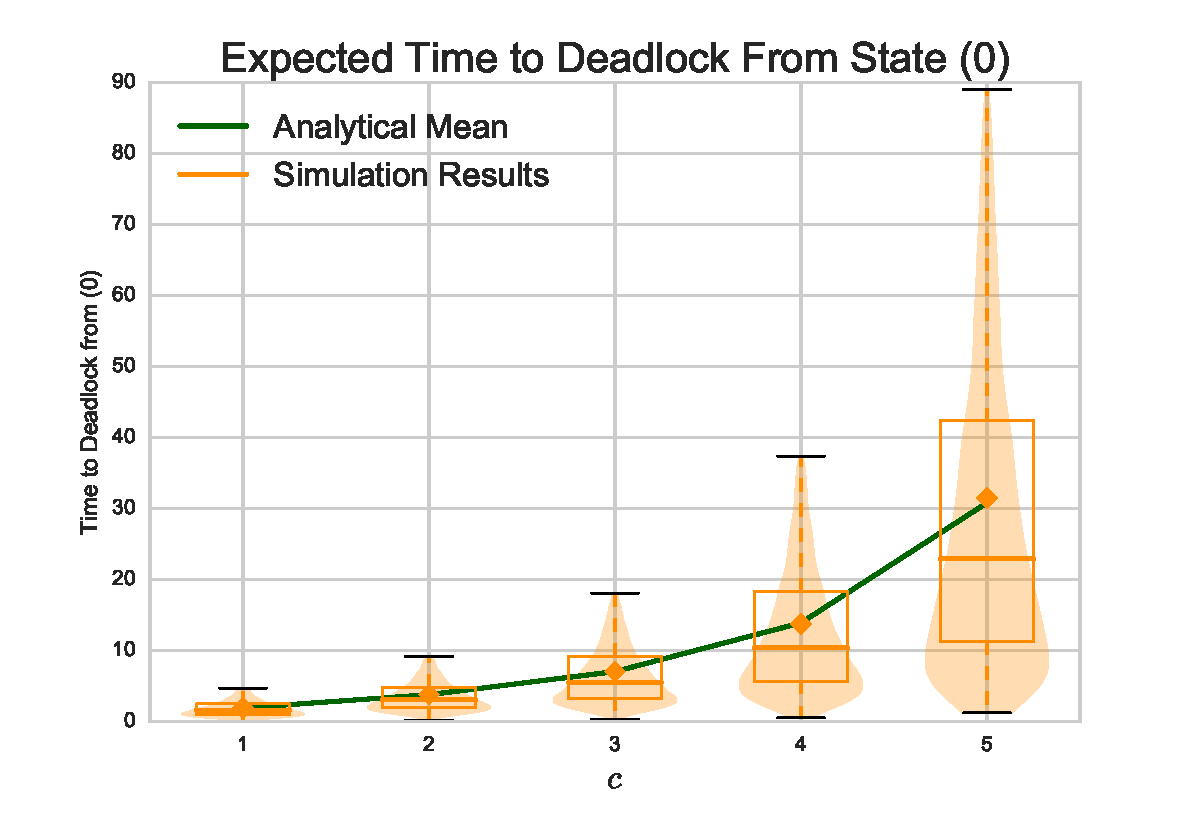
\includegraphics[width=0.5\textwidth]{img/varyc_1Nms}
\end{frame}



% 10th slide, Markov deadlock model 2 Node
\begin{frame}
    \frametitle{Markovian Model of Deadlock}
    \includestandalone[width=\textwidth]{img/2nodemultiserver}\newline
    \center{\LARGE{$(i, j)$}}
\end{frame}


\begin{frame}
\center
\scriptsize \[S = \{(i,j)\in\mathbb{N}^{(n_1+c_1+c_2)\times (n_2+c_2+c_1)} \nonscript\; | \nonscript\; i \leq n_1+c_1+j, \nonscript\; j \leq n_2+c_2+i\}\]

\scalebox{0.8}{\parbox{.5\linewidth}{%
\begin{align*}
  \delta &= (i_2, j_2) - (i_1, j_1)\\
  b_1 &= \max(0, i_1-n_1-c_1)\\
  b_2 &= \max(0, i_2-n_2-c_2)\\
  s_1 &= \min(i_1, c_1)-b_2\\
  s_2 &= \min(i_2, c_2)-b_1\\
\end{align*}
}}


\begin{table}
\begin{center}
\resizebox{\textwidth}{!}{
\begin{tabular}{ l | l | l | l |}
  & $j_1 < n_2 + c_2$ & $j_1 = n_2 + c_2$ & $ j_1 > n_2 + c_2$ \\ \hline
  \rotatebox[origin=c]{90}{$i_1 < n_1 + c_1$} & \begin{tabular}{ l } \color{red} $\Lambda_1$ if $\delta = (1, 0)$ \\ \color{orange} $\Lambda_2$ if $\delta = (0, 1)$ \\ \color{darkgreen} $r_{12}s_1\mu_1$ if $\delta = (-1, 1)$ \\ \color{green} $r_{21}s_2\mu_2$ if $\delta = (1, -1)$ \\ \color{blue} $(1-r_{12})s_1\mu_1$ if $\delta = (-1, 0)$ \\ \color{lightblue} $(1-r_{21})s_2\mu_2$ if $\delta = (0, -1)$ \end{tabular} & \begin{tabular}{ l } \color{red} $\Lambda_1$ if $\delta = (1, 0)$ \\ \color{darkgreen} $r_{12}s_1\mu_1$ if $\delta = (0, 1)$ \\ \color{green} $r_{21}s_2\mu_2$ if $\delta = (1, -1)$ \\ \color{blue} $(1-r_{12})s_1\mu_1$ if $\delta = (-1, 0)$ \\ \color{lightblue} $(1-r_{21})s_2\mu_2$ if $\delta = (0, -1)$ \end{tabular} & \begin{tabular}{ l } \color{red} $\Lambda_1$ if $\delta = (1, 0)$ \\ \color{darkgreen} $r_{12}s_1\mu_1$ if $\delta = (0, 1)$ \\ \color{green} $r_{21}s_2\mu_2$ if $\delta = (0, -1)$ \\ \color{blue} $(1-r_{12})s_1\mu_1$ if $\delta = (-1, 0)$ \\ \color{lightblue} $(1-r_{21})s_2\mu_2$ if $\delta = (-1, -1)$ \end{tabular} \\ \hline
  \rotatebox[origin=c]{90}{$i_1 = n_1 + c_1$} & \begin{tabular}{ l } \color{orange} $\Lambda_2$ if $\delta = (0, 1)$ \\ \color{darkgreen} $r_{12}s_1\mu_1$ if $\delta = (-1, 1)$ \\ \color{green} $r_{21}s_2\mu_2$ if $\delta = (1, 0)$ \\ \color{blue} $(1-r_{12})s_1\mu_1$ if $\delta = (-1, 0)$ \\ \color{lightblue} $(1-r_{21})s_2\mu_2$ if $\delta = (0, -1)$ \end{tabular} & \begin{tabular}{ l } \color{darkgreen} $r_{12}s_1\mu_1$ if $\delta = (0, 1)$ \\ \color{green} $r_{21}s_2\mu_2$ if $\delta = (1, 0)$ \\ \color{blue} $(1-r_{12})s_1\mu_1$ if $\delta = (-1, 0)$ \\ \color{lightblue} $(1-r_{21})s_2\mu_2$ if $\delta = (0, -1)$ \end{tabular} & \begin{tabular}{ l } \color{darkgreen} $r_{12}s_1\mu_1$ if $\delta = (0, 1)$ \\ \color{green} $r_{21}s_2\mu_2$ if $\delta = (1, 0)$ \\ \color{blue} $(1-r_{12})s_1\mu_1$ if $\delta = (-1, 0)$ \\ \color{lightblue} $(1-r_{21})s_2\mu_2$ if $\delta = (-1, -1)$ \end{tabular} \\ \hline
  \rotatebox[origin=c]{90}{$i_1 > n_1 + c_1$} & \begin{tabular}{ l } \color{orange} $\Lambda_2$ if $\delta = (0, 1)$ \\ \color{darkgreen} $r_{12}s_1\mu_1$ if $\delta = (-1, 0)$ \\ \color{green} $r_{21}s_2\mu_2$ if $\delta = (1, 0)$ \\ \color{blue} $(1-r_{12})s_1\mu_1$ if $\delta = (-1, -1)$ \\ \color{lightblue} $(1-r_{21})s_2\mu_2$ if $\delta = (0, -1)$ \end{tabular} & \begin{tabular}{ l } \color{darkgreen} $r_{12}s_1\mu_1$ if $\delta = (0, 1)$ \\ \color{green} $r_{21}s_2\mu_2$ if $\delta = (1, 0)$ \\ \color{blue} $(1-r_{12})s_1\mu_1$ if $\delta = (-1, -1)$ \\ \color{lightblue} $(1-r_{21})s_2\mu_2$ if $\delta = (0, -1)$ \end{tabular} & \begin{tabular}{ l } \color{darkgreen} $r_{12}s_1\mu_1$ if $\delta = (0, 1)$ \\ \color{green} $r_{21}s_2\mu_2$ if $\delta = (1, 0)$ \\ \color{blue} $(1-r_{12})s_1\mu_1$ if $\delta = (-\min(b_1+1,b_2+1), -\min(b_1,b_2+1))$ \\ \color{lightblue} $(1-r_{21})s_2\mu_2$ if $\delta = (-\min(b_1+1,b_2), -\min(b_1+1,b_2+1))$ \end{tabular} \\ \hline
\end{tabular}
}
\end{center}
\end{table}
\end{frame}

\begin{frame}
    \begin{figure}
    \includestandalone[width=0.95\textwidth]{img/MC2nodemultiserv}
    \end{figure}
\end{frame}

\begin{frame}
    \frametitle{Times to Deadlock}
    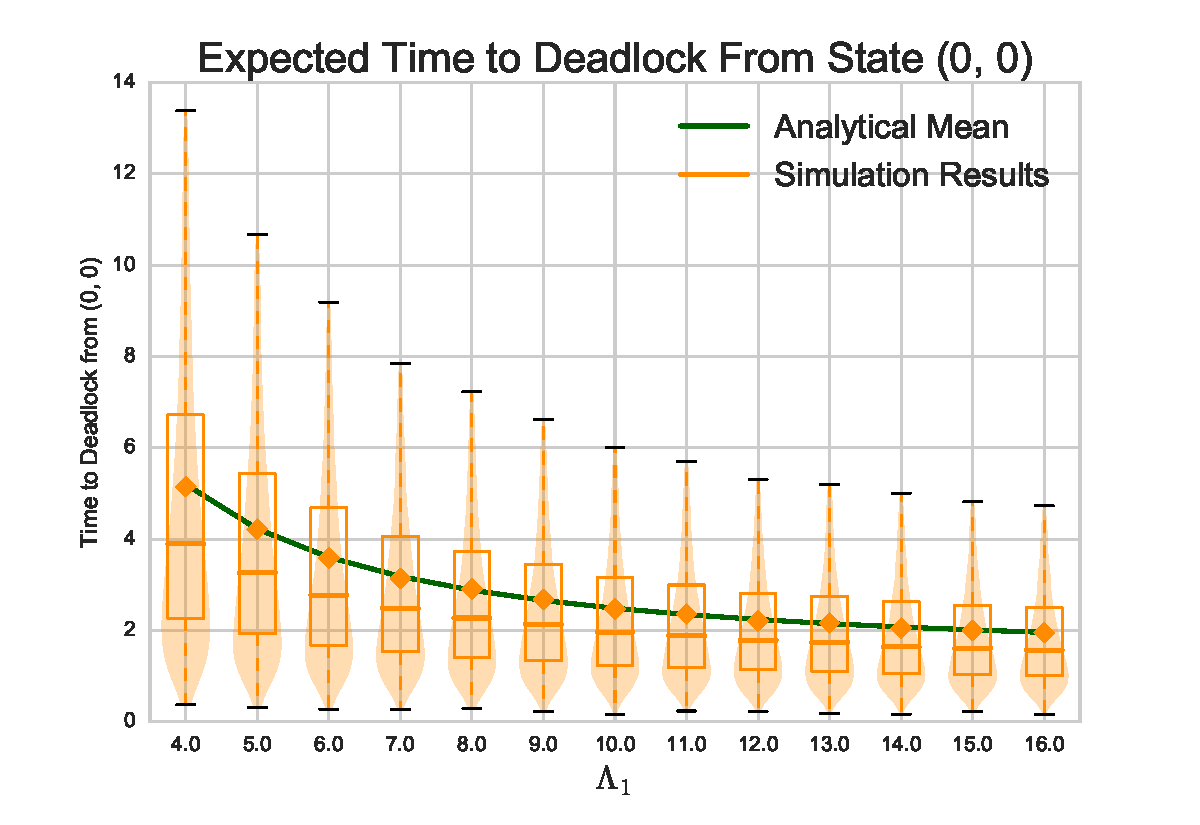
\includegraphics[width=0.5\textwidth]{img/varyL1_2Nms}
    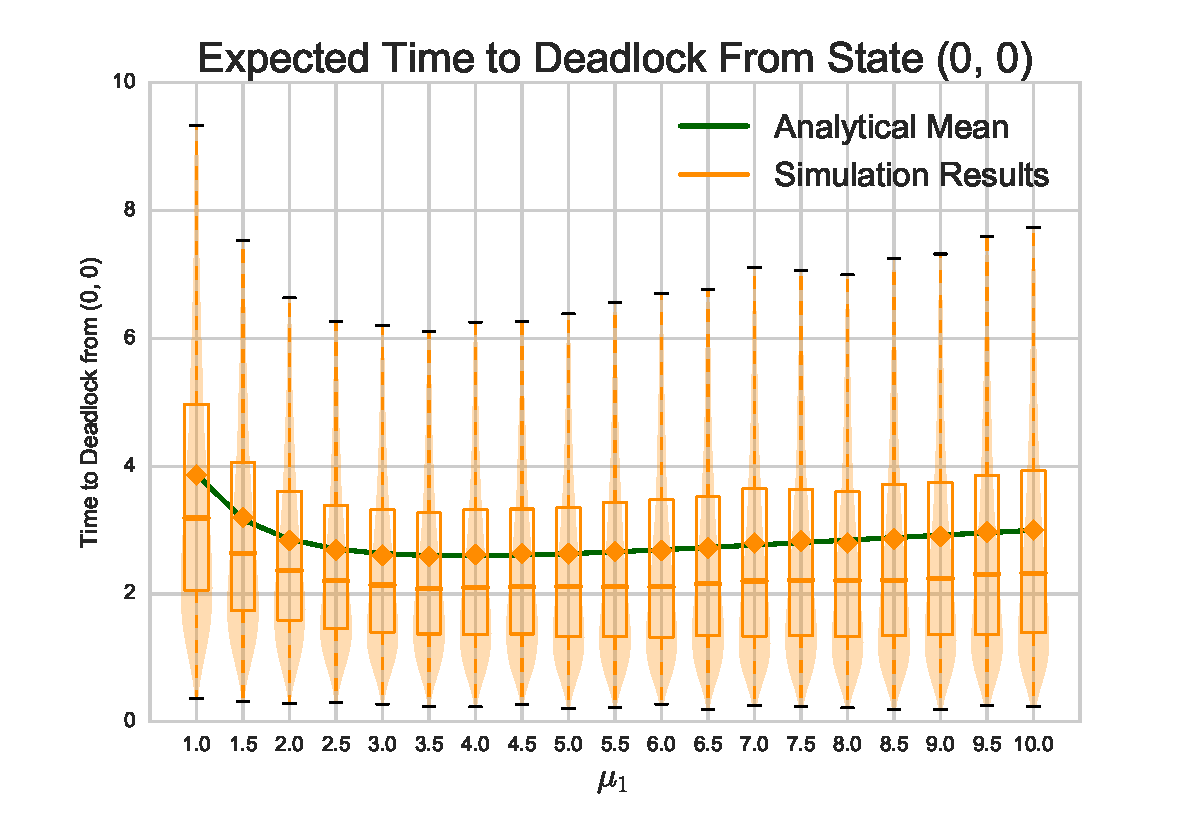
\includegraphics[width=0.5\textwidth]{img/varymu1_2Nms}\newline
    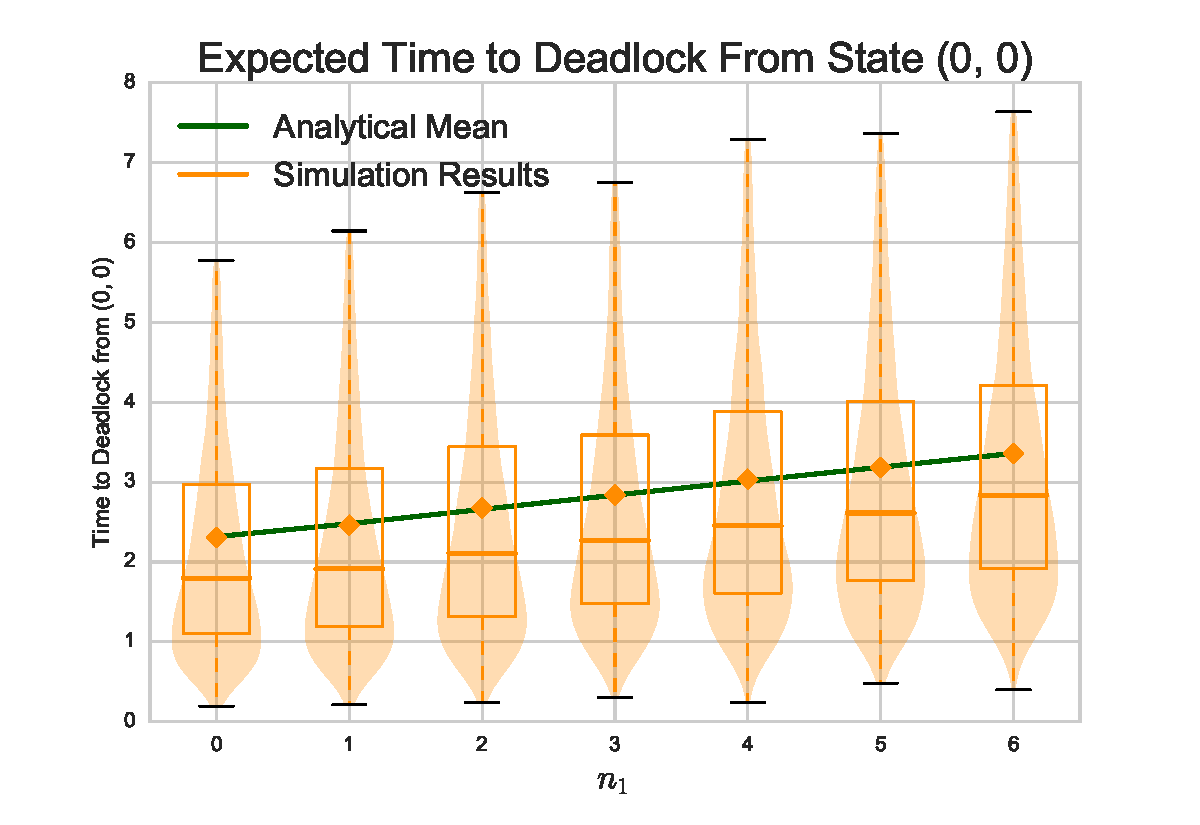
\includegraphics[width=0.5\textwidth]{img/varyn1_2Nms}
    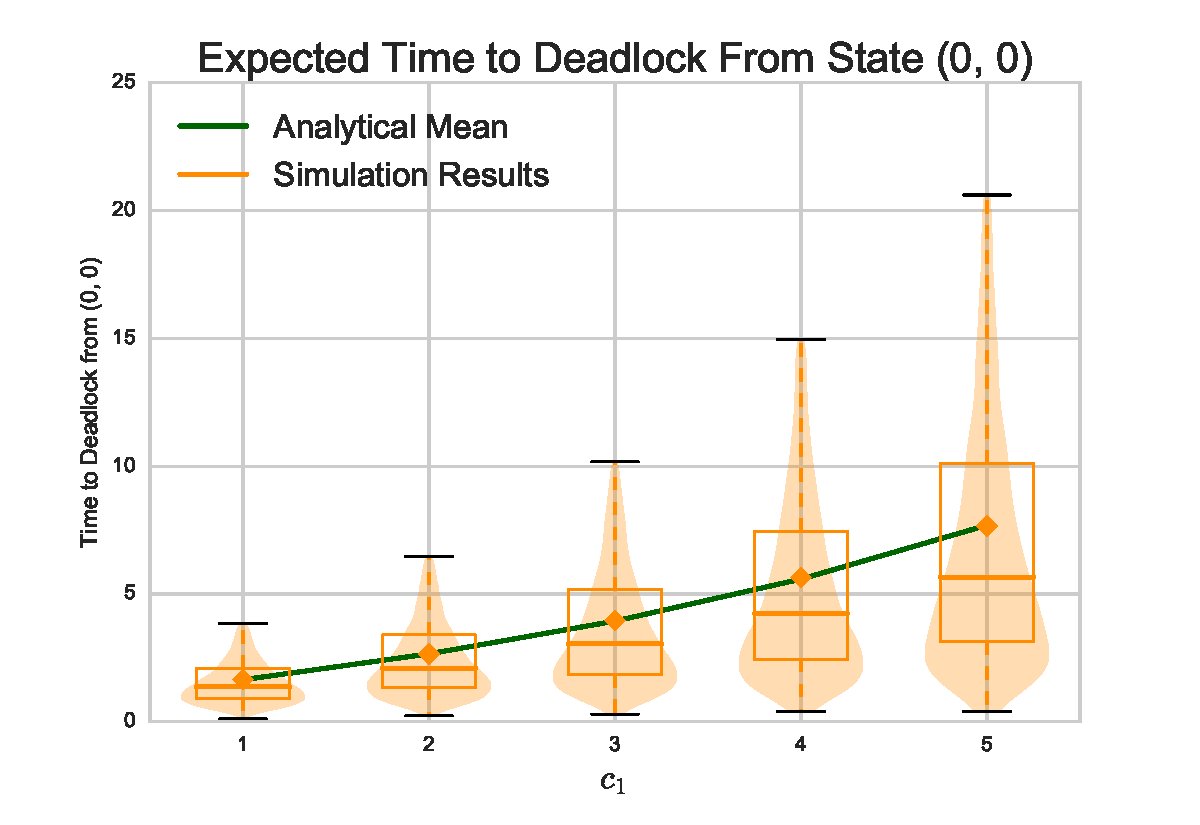
\includegraphics[width=0.5\textwidth]{img/varyc1_2Nms}
\end{frame}


% 11th lide, Markov deadlock model 2 Node self loops
\begin{frame}
    \frametitle{Markovian Model of Deadlock}
    \includestandalone[width=\textwidth]{img/2nodefeedbackexample}\newline
    \center{\LARGE{$(i, j)$}}
\end{frame}


\begin{frame}
\center
\scriptsize \[S = \{(i,j)\in\mathbb{N}^{(n_1+2\times n_2+2)} \nonscript\; | \nonscript\; 0 \leq i + j \leq n_1 + n_2 + 2\}\cup\{(-1), (-2), (-3)\}\]
Define $\delta = (i_2, j_2) - (i_1, j_1)$\newline\newline
\tiny{
  $q_{(i_1, j_1),(i_2, j_2)} = \left\{
  \begin{matrix*}[ r ]
    \left. \color{red} \begin{matrix*}[ r ]
      \Lambda_1 & \text{if } i_1 \leq n_1 \\
      0 & \text{otherwise}
    \end{matrix*} \right\} & \color{red} \text{if } \delta = (1, 0)\\
    \left. \color{orange} \begin{matrix*}[ r ]
      \Lambda_2 & \text{if } j_1 \leq n_2 \\
      0 & \text{otherwise}
    \end{matrix*} \right\} & \color{orange} \text{if } \delta = (0, 1) \\
    \left. \color{blue} \begin{matrix*}[ r ]
      (1 - r_{12})\mu_1 & \color{blue} \text{if } j_1 < n_2 + 2 \\
      0 & \text{otherwise}
    \end{matrix*} \right\} & \color{blue} \text{if } \delta = (-1, 0) \\
    \left. \color{lightblue} \begin{matrix*}[ r ]
      (1 - r_{21})\mu_2 & \text{if } i_1 < n_1 + 2 \\
      0 & \color{lightblue} \text{otherwise}
    \end{matrix*} \right\} & \color{lightblue} \text{if } \delta = (0, -1) \\
    \left. \color{darkgreen} \begin{matrix*}[ r ]
      r_{12}\mu_1 & \text{if } j_1 < n_2 + 2 \text{ and } (i_1, j_1) \neq (n_1+2, n_2) \\
      0 & \text{otherwise}
    \end{matrix*} \right\} & \color{darkgreen} \text{if } \delta = (-1, 1) \\
    \left. \color{green} \begin{matrix*}[ r ]
      r_{21}\mu_2 & \text{if } i_1 < n_1 + 2 \text{ and } (i_1, j_1) \neq (n_1, n_2+2)\\
      0 & \text{otherwise}
    \end{matrix*} \right\} & \color{green} \text{if } \delta = (1, -1) \\
    0 & \text{otherwise}
  \end{matrix*} \right.$\newline\newline

  $q_{(i_1, j_1), (-1)} = \left\{
  \begin{matrix*}[ r ]
    \color{magenta!50} r_{11}\mu_1 & \color{magenta!50} \text{if } i > n_1 \text{ and } j < n_2 + 2 \\
    0 & \text{otherwise}
  \end{matrix*}
  \right.$\newline

  $q_{(i_1, j_1), (-2)} = \left\{
  \begin{matrix*}[ r ]
    \color{violet!50} r_{22}\mu_2 & \color{violet!50} \text{if } j > n_2 \text{ and } i < n_1 + 2 \\
    0 & \text{otherwise}
  \end{matrix*}
  \right.$\newline

  $q_{(i_1, j_1), (-3)} = \left\{
  \begin{matrix*}[ r ]
    \color{green} r_{21}\mu_2 & \color{green} \text{if } (i, j) = (n_1, n_2 + 2) \\
    \color{darkgreen} r_{12}\mu_1 & \color{darkgreen} \text{if } (i, j) = (n_1 + 2, n_2) \\
    0 & \text{otherwise}
  \end{matrix*}
  \right.$\newline

$q_{-1, s} = q_{-2, s} = q_{-3, s} = 0$
}
\end{frame}


\begin{frame}
    \begin{figure}
    \includestandalone[width=0.95\textwidth]{img/markov_chain_feedback}
    \end{figure}
\end{frame}

\begin{frame}
    \frametitle{Times to Deadlock}
    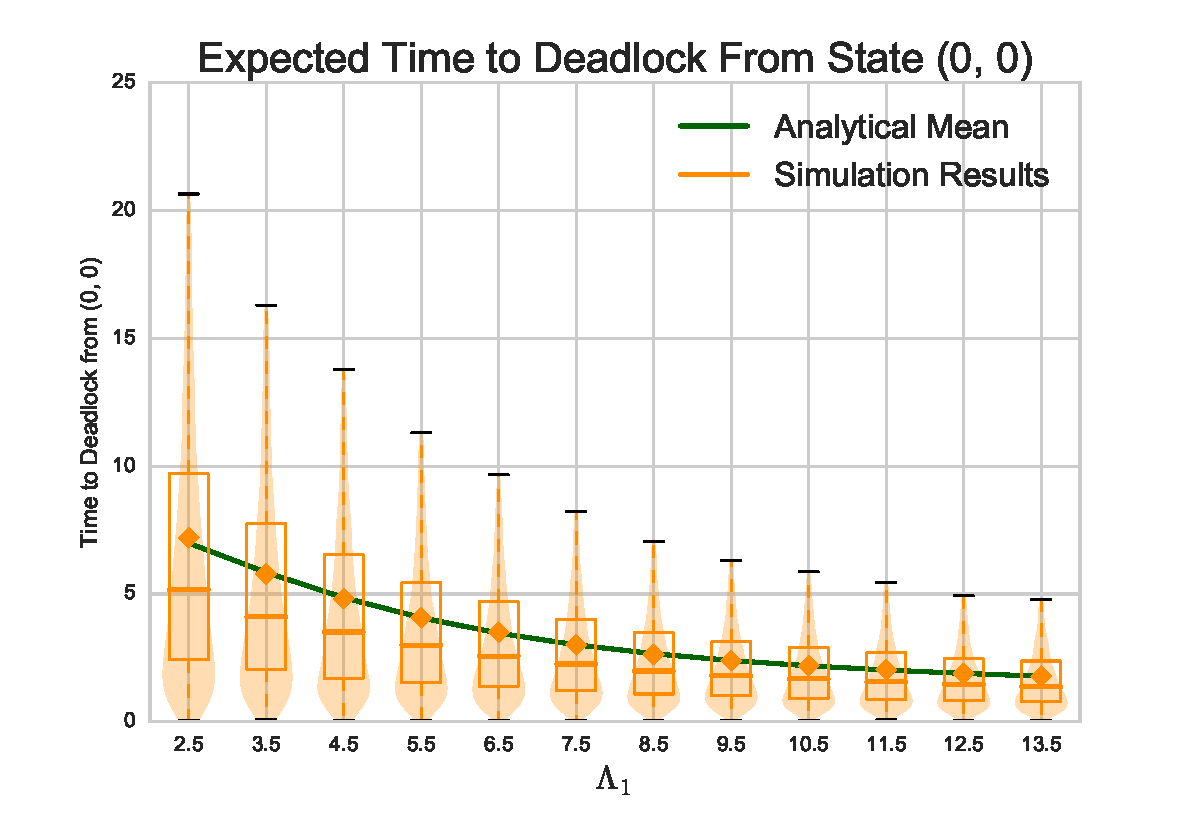
\includegraphics[width=0.5\textwidth]{img/vary_L1fb}
    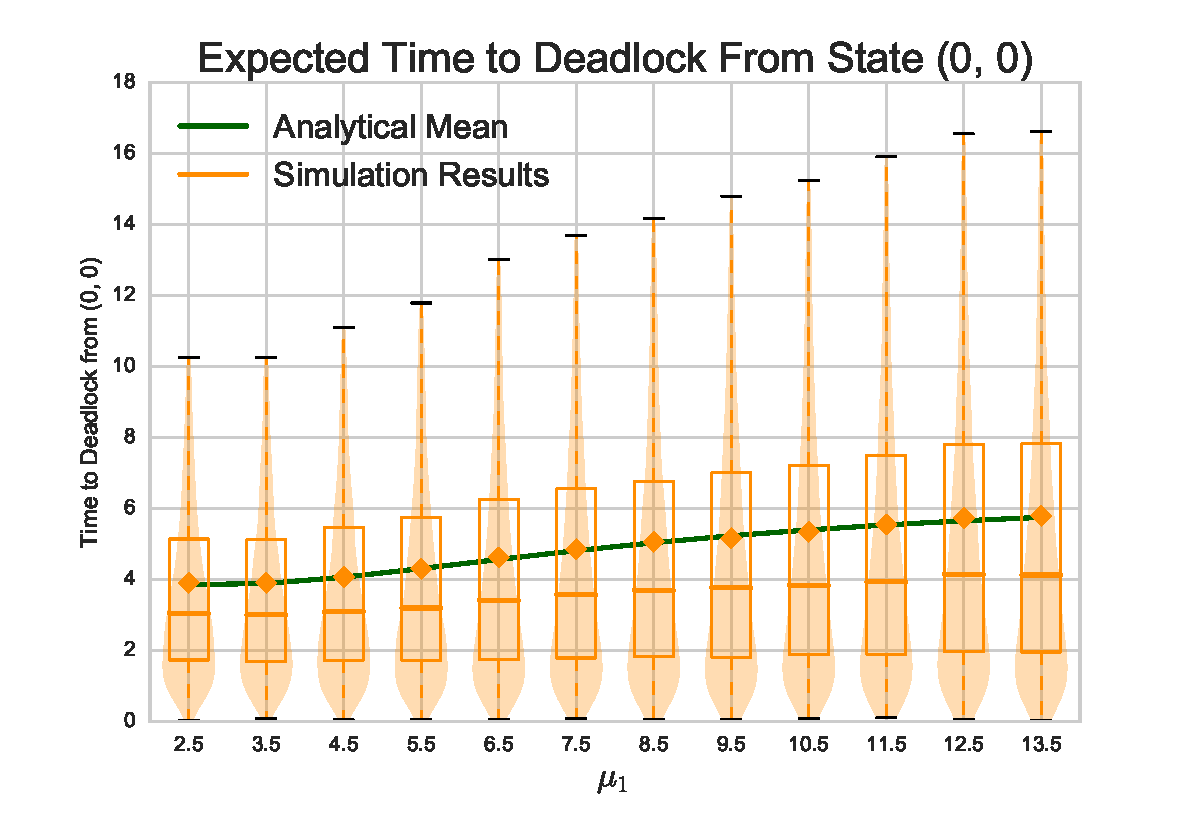
\includegraphics[width=0.5\textwidth]{img/vary_mu1fb}\newline
    \centering
    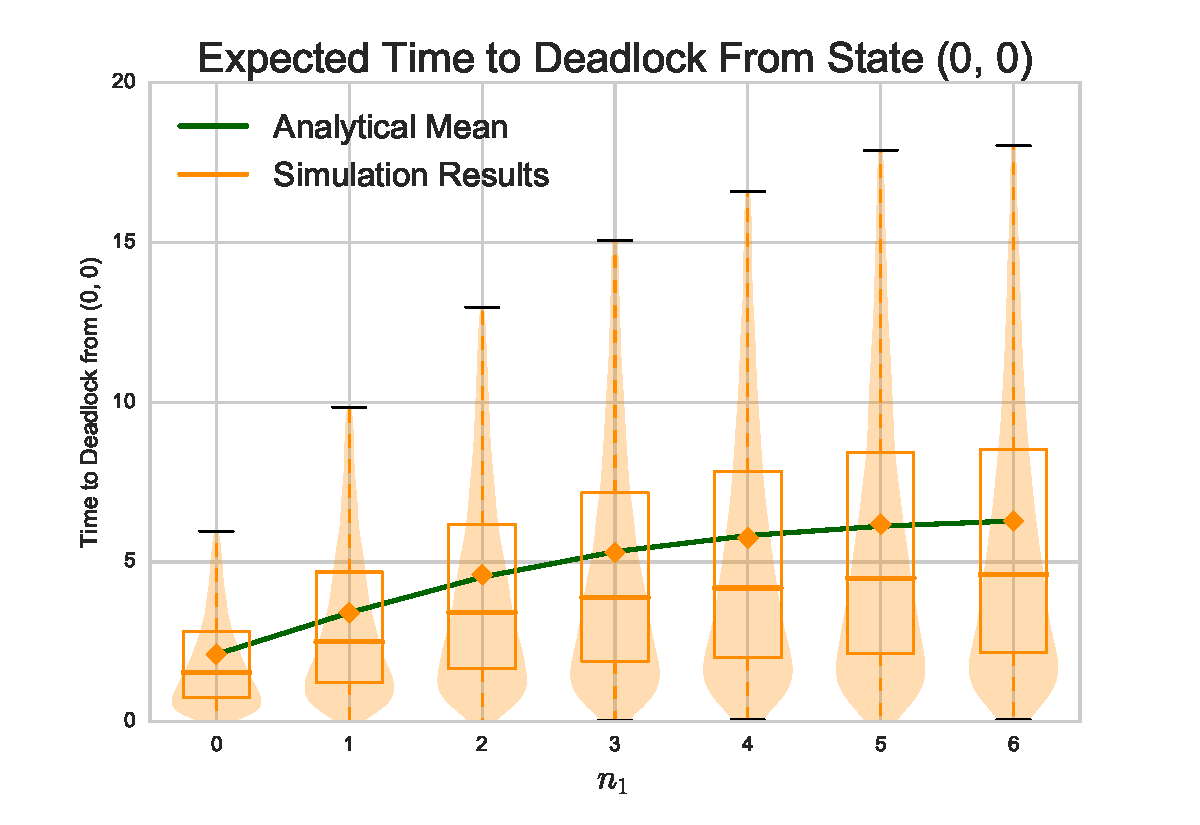
\includegraphics[width=0.5\textwidth]{img/vary_n1fb}
\end{frame}

% 12th slide, remind of healthcare motivation... future work
\begin{frame}
\frametitle{Summary}
\begin{block}{Summary}
\begin{itemize}
\item Investigate deadlock in open restricted queueing networks, especially the time until deadlock occurs.
\item Method of detecting deadlock in discrete event simulations of queueing networks.
\item Three Markov models of deadlocking queueing networks.
\end{itemize}
\end{block}

\begin{block}{To Do...}
\begin{itemize}
\item Build and parameterise patient flow networks from data.
\item Use queueing network analysis and simulation to investigate impact of the OPICP.
\item Determine the OPICP's effect on demand and workforce needs.
\end{itemize}
\end{block}
\end{frame}


% Thank you slide.
\begin{frame}
    \frametitle{Thank You}
    palmergi1@cardiff.ac.uk
\end{frame}

\end{document}
